% !Tex root = main.tex
\documentclass{article}
\usepackage{graphicx}

\title{On the factors describing flowstate; A cognitive perspective}
\author{Jimmy Zeng}

\usepackage[backend=biber,style=apa]{biblatex}
\addbibresource{works_parencited.bib}

% Are you being assessed in 2027 or later, so that the new syllabus applies? What title-page details do you still need (student code, submission date, and final word count)?

\begin{document}
\maketitle
\tableofcontents
\section{Introduction}

% What do you want your main research question to be? (Try choosing one main factor, such as mood or time of day, and name the exact group of students you want to study.)
    
In an increasingly digital society, many teenagers and young adults find issues struggling to focus academically as distractions become ever more prevalent, many new terms such as "flow state" and the state of being "locked in" having increasingly used in social media platforms describe "flow", or, the mental state of total deep engrossment/absorption in a cognitive work and an ensuing loss of self-consciousness.\parencite{Mazid2024} This state is linked to an optimal improvement/learning schedule\parencite{Mazid2024}. %better word it?
And hence, in the contemporary world, this is a particularly an important field of research as our target population of teenagers, given too many choices in life, would find it easier to engage in activities such as watching television, "doomscrolling", and gaming due to the lack of pressure for teenagers to doing "challenging activities that can teach and improve new skills" \parencite{Schwartz2000} \parencite{Mazid2024}. In this stage in life according to piaget's theory of development teenagers are transitioning into higher-order thinking and requires a lot of heavy learning to occur, hence, it is important for them to engage in skill learning as it is a critical developmental stage in human life. 
'Being in the state of flow meant having an optimal experience which has been referred to as “the bottom line of existence (because) without it there would be little purpose in living.”.' \parencite{Mazid2024}


Modern research has identified 9 characteristics of flow the flow experience. The challenge skill balance is often considered the backbone of flow research. This characteristic suggests that flow is reached when the perceived challenge of the task matches the skill level of the participant. Illustrated in figure \ref{fig:challenge-skill}. This parallels to Vygotsky's "Zone of Proximal Development" which is being in a skill level where it requires help from a more knowledgable other rather than being impossible nor able to be done without any external assistance.
\begin{figure}[htbp]
    \center
    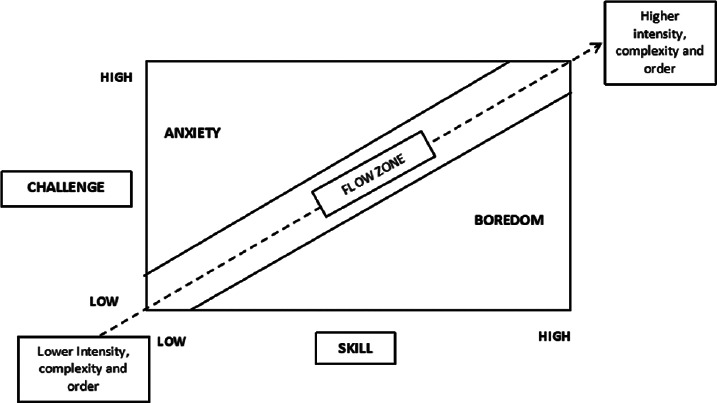
\includegraphics[width=\textwidth]{challenge skill balance}
    \caption{The challenge-skill balance model of flow state \parencite{Mazid2024}}
    \label{fig:challenge-skill}
\end{figure}

However, many other factors were later discovered in relating to flow, such as perceived control. However, this does not necessarily mean the advancement in resources. For instance, giving one a calculator in a math test, may increase their "perceived control", but that is because it does really increase their control in their situation, similar to having access to more money/funding to accomplish a task. And it is imperative that we operationalize perceived control carefully.

Hence, this research will focus on the effect of perceived control on the magnitude of flow measured as a classification based on absorption, timelessness and effort. %Somehow bold this


\section{Methodology}

\subsection{Sampling Population}
% What research method have you chosen, and why does it fit your question? (For example, will it let you compare groups, look for a relationship, or understand students' experiences in depth?)
Our population will be chosen based on opportunity sampling. We will choose 10th grade students based on their grades in humanities class since 10 grade students are relatively blithe compared to us IB die-hards, which satisfies the criterion for low pressure for work, meaning they just so happen to have more reason to need to improve their skills in this stage of development. %definitely can be written betterly, somehow tie this back into impact. its like yeah, it is important to learn and improve their skills like we mentioned earlier, this is literally a perfect example of that. but i mean in a more formal way.
According to Csikszentmihalyi's model, the skill-challenge balance plays an important role in achieving flow state, % Word better?
therefore it is important that we establish a population of similar skill level, and the challenge will be the same as we will maintain same procedure for each trial.
It is known last year that we were "voluntold" to be subject to the senior's dreadful experiments to get them their diploma. A similar setup should be possible (had the ib maintained allowing psychological experimenting and) if our school were open to coordination. 
Hence, in order for the skill level to stay constant based on Csikszenmihalyi's model we would choose a sample population based on stratified sampling on the same humanities class. It is possible to obtain access to their grades having expressed our dire situation. If rejected like college applications, we may resort to systemic sampling by engaging in the ethically ilicit activity known as being familiar with students in their grade to know who are the high-achieving students and who are not and then stratifically sample based on the best of our ability. [yeah definitely need work on wording that]

\subsection{Ethical Considerations}
It will be disclosed to each participant that at any point in the study they have the right to withdraw, informing that their data is to be deleted in such cases.

As this is noted, we will provide a consent form that will include all potential negative effects of such experimenting. Which includes:
\begin{itemize}
    \item Pressure to complete the task (may exist in high-achieving students)
    \item Slight embarrasment (from watching yourself, but this will not be disclosed on the form such that they will not be distracted from the task at hand[but this whole part should be worded better])
\end{itemize}

It is known that all Psychological experimenting should attempt to result in maximising benefit and minimizing harm, referred to as "beneficence". This suggests that our independent variable should be unipolar, controlling the magnitude of perceive control rather than purely depriving them of control. This would theoretically only result in effect would be varying magnitudes of improvement rather than any deprovements. 

Minor levels of deception will be used, since we will record their screen during work as well as provide a facecam to refer to afterwards. This will be reduced to "The program will be collecting data during work" without informing them of face/screen recording such that they may focus on the task at hand.

%Mention that the lack of a screen recording was a weak point in the experiment of the study


% Hence as we are able to find the ratio between change in perceived control and change in magnitude of the flow state, we should be able to extrapolate that a deprivation of control would result in a deprovement.
% \begin{figure}[htbp]
%     \center
%     \begin{tikzpicture}
%         \begin{axis}
%
%         \end{axis}
%     \end{tikzpicture}
%     \caption{An illustration of extrapolating deprovement based on improvement curve}
%     \label{fig:improvement/deprovement}
% \end{figure}

\subsection{Changing the independent variable}

The indepedent variables of "perceived control" has nuance, in one hand, it is their ability to choose what prompts to work on or what they are most confortable with, but what if they were unfamiliar with any of them. They would end up in (there was an experiment on mind field youtube that was like if someone choose it for you you would feel like you did better, but if you choose yourself you would feel worse, I'm certain there is a technical name for that)
% What ethical issues could come up in your study, and what will you do about each one? (Consider consent or assent, parental permission if needed, withdrawal, privacy of recordings, confidentiality, discomfort, and debriefing.)
    
\subsection{Designing the Data Collection}

% What one data collection tool will you create to measure flow? (For example, a questionnaire, rating scale, interview schedule, or observation checklist with at least five items.)

Many methods of data collection for flow has been used such as the four-channel model ratio of challenge and skill, and a classification based on ratings of absorption, timelessness and effort \parencite{AINLEY2008109}. However, we will focus on using a classification based on absorption, timelessness and effort. Since this better describes the effects of flow rather than the theoretical preconditions that affect flow such as skill-challenge balance. For instance, being in flow, one would certainly feel absorbed in the task, as per the definition of flow. % write the definition of flow
However, it does not mean that this is inherently caused by a equal balance of challenge and skill. After all, we are interested in optimizing the beneficial effects of flow, hence, we must resort to the definition of the effects of flow rather than the theoretical preconditions of flow.

% Is there an existing flow measure or model you can use to guide your tool? What parts of flow does it measure, and why do they fit your question and your students?

Operationalized variables: The level of flow should be experimentally determined by the following factors
% What would count as evidence of flow in your study? (Choose clear signs or scores that measure flow separately from mood, effort, task success, or time spent working.)
Potential speculated factors affecting it
% Which factor is the main focus, and which ones are just possible confounding variables? (For example, where do sleep, food, prior activity, task interest, and skill level fit?)

The tool itself:
% Which option below is your overall research method, and which is the tool used within it? How will that tool give you evidence that answers your question?
\begin{enumerate}
    \item questionaire/survey
    \item experiment
    \item observation
    \item interview
\end{enumerate}
you can only do 5 items anyways
% Have you noted that the current guide asks for at least five items, not only five? Will you put the complete tool in the appendix?

the explanation of the decisions 
explain, not describe 
it has to be effective, valid, and reliable
your tool needs to match the population. it has to be relevant to the population
% Why have you included each item in the tool, and what will make the tool trustworthy? (Explain what each item measures and how it is scored; check that the wording is clear and neutral and that any footage is judged using a consistent checklist rather than personal impressions.)

Survey
% If you choose a survey or questionnaire, how will it measure what students experienced during the task rather than only what they generally believe about flow?

potential challenges
% What could make your data misleading, and how could you reduce each problem? (Choose only the challenges that genuinely fit your study, explain how they could affect the findings, and say what limitation would remain afterward.)

I think I will be doing experiment, doing an assignment, throughout different times of the day. and recording factors such as food consumption, what you were doing earlier (productive/relaxing work), etc. And then seeing what factors most visibly affected the flowstate or if they even were able to achieve flowstate we use a standardized test I forgot what it was called but I am certain there are many ways of doing it. if they didn't achieve flowstate, explain why they didn't
% What is the standardized measure you were thinking of, and how would you use it here? (Find its name and source, check that it suits your students, decide what counts as higher or lower flow, and consider whether sleep, food, earlier activities, or schedules could explain a time-of-day difference.)


\section{Discussion}
% What might you find? (Describe what a positive, negative, mixed, or unclear result would look like in your measurements, how it would answer your question, how it connects to your two studies, and what else might explain it.)
    
Discussion of the potential findings of the investigation and the implications for policyt/practice
how it can potentially be used for making policies of the school for instance.
% If your expected finding appeared, what could a school realistically change in its policy or everyday practice, and how might that help these students? What should the school be cautious about before applying it?
*start with a paragraph
bias:
\begin{enumerate}
    \item how might've bias influenced
    \item your personal history (are you involved?)
\end{enumerate}
% How might your own experiences or beliefs about focus, mood, and being ``locked in'' have shaped this proposal? (Consider your topic, expected result, question wording, observation of footage, or interpretation.)
% What could you do to reduce this researcher bias, and how might it still affect the investigation even after that precaution?
each criteria/section should have 3 paragraphs

potential findings are described in detail, and implications for poliicy/practice

relevant examples of how researcher bias is influenced (one is enough, I can talk about confirmation bias)

one relevant additional research method with reference to increasing the understanding of the area of investigation
% What different research method could explore the same topic? What would it help you understand about students' flow that your main method might miss, and what limitation would it bring?

% Final check: have you included full references and an appendix with your complete tool, and is the assessed report within 2,200 words?

\printbibliography

\end{document}
